\subsection{AI Setup}

\textbf{Program Flow:}
The program is set up in a way that adheres to the following flow structure:

%
%%image here ./kkimgs/ProgramFlow

\begin{figure}[position = here]
	\begin{centering}
		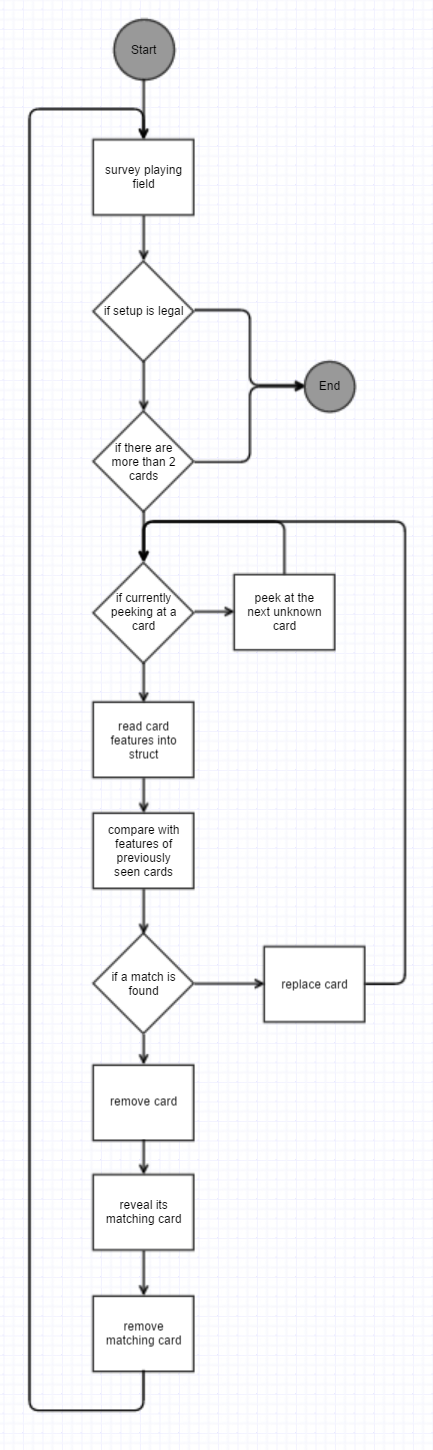
\includegraphics[scale=0.75]{./kkimgs/ProgramFlow.png}\\
		\caption[]{\textit{Program Flow Diagram\label{prgflw}}}
	\end{centering}
\end{figure}

This structure in Fig.\ref{prgflw} focuses on claiming a matching pair as soon as it is found.

\textbf{Game Modes:}
Consider the logic table in Fig.\ref{gmmds} which shows us 16 different numbers that can be expressed as a single character where the the 4 right hand bits represent a flag value for what should be compared in each run of the game based on the game mode that is selected. The reason for this comparison structure is that if individual flags are set high we would have to poll all the flags but by using bits in a character as a flag system we can simply compare with a final value that we expect to see which reduces the number of flag checking to a single poll irrespective of the number of factors that need to be compared. This maximises the scalability of this program to series of cards with many more differences.

It's important to note that this compare function is designed to be modified for the game Set. In the game Concentration we use a Game Mode that's specified in code that masks the bits in a way that we only get identical pairs. Whereas to develop this for set we would have to see assign a "score" for each set that was found and at the end of examining EVERY card on the field figure out the combinations that will maximize the score that can be made from the series of cards at hand. In this setup we had Game Mode 11 as we couldn't acquire colour images from the camera. This game mode will accept sets of cards that have the same Shape, Filler, and Count.
%image here ./kkimgs/GameModes
\begin{figure}[position = here]
	\begin{centering}
		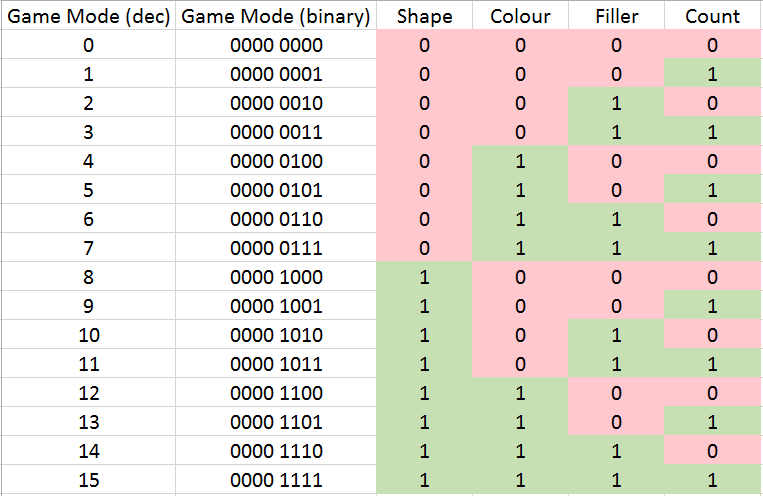
\includegraphics[scale=0.6]{./kkimgs/GameModes.png}\\
		\caption[]{\textit{Game Modes\label{gmmds}}}
	\end{centering}
\end{figure}

	
\textbf{Card Data Structure}
One of the more important parts of the setup is that the program is able to see what it considers a set of cards where each card has:

\begin{itemize}
	\item X Coordinates
	\item Y Coordinates
	\item Orientation
	\item Shape
	\item Colour
	\item Filler
	\item Count
\end{itemize}

This makes it very easy to address individual traits on any set of cards. This needs to also have a trait that links it to other cards that it could form a set with and the score potential 
